\chapter{弱衍射和重叠：先写对似然}
\section{负强度并不意味着负光子}
若背景扣除后的观测满足 $y\sim\mathcal N(I,\sigma^2)$，即使物理信号 $I\ge0$，也可能测得 $y<0$。对于 $I=0$，
\begin{equation}
 \E(y)=0,\qquad \E\{\max(y,0)\}=\frac{\sigma}{\sqrt{2\pi}}.
\end{equation}
所以把所有负观测裁成零会人为增加弱反射的平均信号。若进一步只保留 $y/\sigma$ 大的行，入选样本还会偏向正噪声。French--Wilson 方法讨论的是如何结合统计先验估计振幅，而不是允许把先验后的振幅当成新的独立测量\cite{french1978}。

本软件在 $F^2$ 精修中保留所有有效的带符号强度。相位初始化可以构造非负振幅作为数值起点，但新的混合算法随后使用原始 $y,\sigma$ 的强度似然。真实光子计数则使用非负计数模型，两者的“非负”作用于不同对象。
\begin{figure}[!htbp]
\centering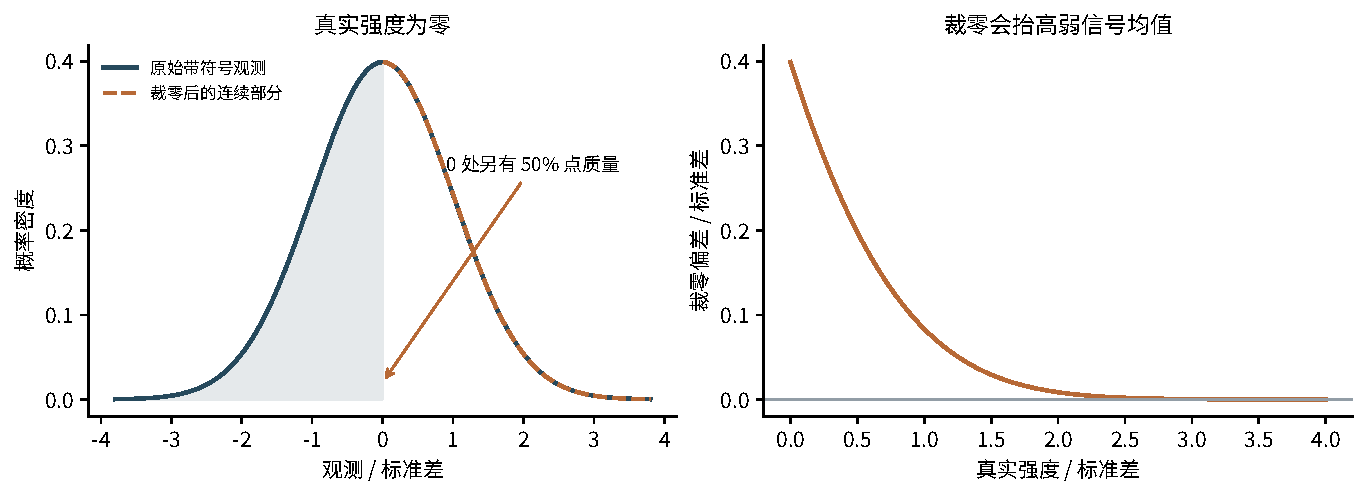
\includegraphics[width=0.94\textwidth]{figures/03_weak_bias.pdf}
\caption{零真实信号的高斯教学模型。负观测是噪声模型的一部分；裁零后在原点形成点质量，均值由零变为 $0.399\sigma$。右侧展示不同真实信号下裁零估计的偏差。曲线来自解析公式，不是软件成功率。}
\end{figure}

\section{高斯像素的背景消元}
令同一像素组内的模型为
\begin{equation}
 y=PI+B_g\beta+\varepsilon,\qquad \varepsilon\sim\mathcal N(0,W^{-1}).
\end{equation}
$I$ 是所有反射分量的强度，$B_g\beta$ 是共同背景。白化后 $\widetilde y=W^{1/2}y$、$\widetilde P=W^{1/2}P$。若 $Q_b$ 的列张成 $W^{1/2}B_g$，消去线性背景等价于
\begin{equation}
 \min_\beta\|W^{1/2}(y-PI-B_g\beta)\|^2
 =\|(I-Q_bQ_b^{\mathsf T})(\widetilde y-\widetilde PI)\|^2.
\end{equation}
实现中不显式生成像素数平方的投影矩阵。对增广设计矩阵按行分块作 QR 消元，再对小矩阵分解，可得到
\begin{equation}\boxed{\quad\chi^2(I)=\|RI-z\|^2+c.\quad}\label{eq:sufficient}
\end{equation}
$R,z,c$ 对任意候选 $I$ 都保留相同目标值。$c$ 不影响最优结构，却影响完整的拟合统计；比较模型或报告像素残差时不能丢掉它。这种方法属于可分离变量消元与平方根最小二乘的应用\cite{golub1973}。

QR 的价值还在于避免先形成 $P^{\mathsf T}WP$。后者将条件数平方；高度重叠时，浮点误差会更早破坏最弱的信息方向。新接口同时保留小矩阵、零空间和原始强度单位。

\section{可辨识性比强弱更基本}
对两个形状完全相同的峰，$P=[p,p]$，像素只依赖 $I_1+I_2$。无论曝光多少次，都不能仅靠这组像素区分 $(I_1,I_2)$ 和 $(I_1+t,I_2-t)$。它的零空间包含 $(1,-1)$。

对于归一化后相关系数为 $\rho$ 的两列，简化信息矩阵的两个特征值正比于 $1+\rho$ 与 $1-\rho$。当 $\rho\to1$，总量方向仍有信息，差量方向的信息趋于零。这个结论解释了为什么某些很强的重叠点反而比孤立弱点更难拆分。
\begin{figure}[!htbp]
\centering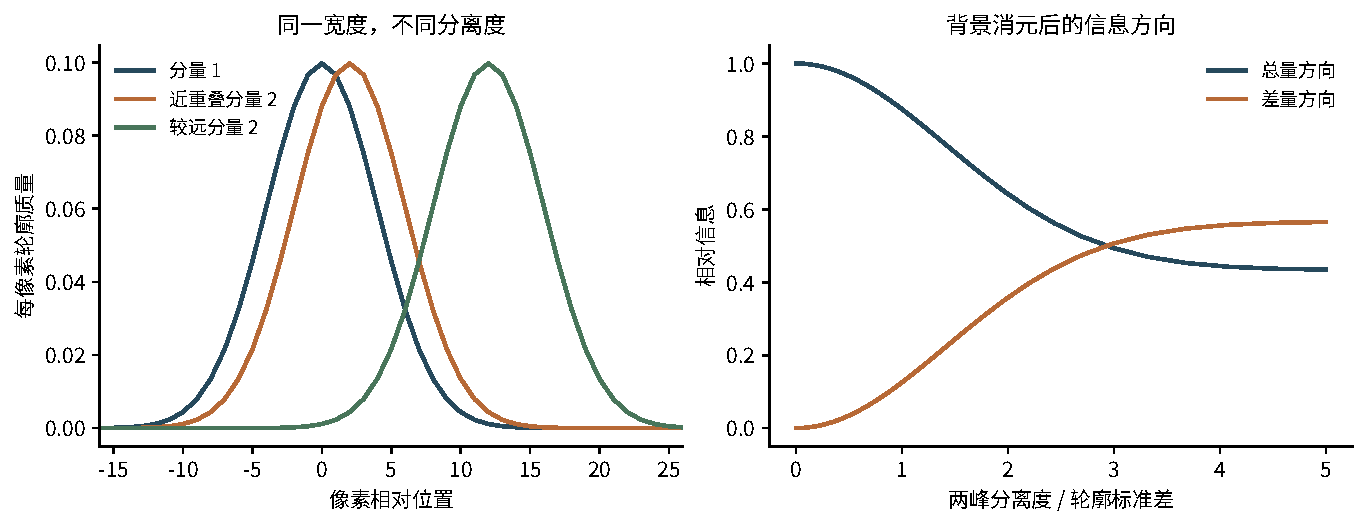
\includegraphics[width=\textwidth]{figures/04_overlap_information.pdf}
\caption{两个高斯轮廓随分离度变化的可辨识性。左侧是轮廓；右侧是背景消元后差量与总量的信息变化。完全重合时差量不可辨识。数据由新压缩接口对固定轮廓计算，所有幅度仍可取正或负。}\label{fig:overlap}
\end{figure}

因此分流依据包括探测器噪声类型、轮廓几何和信息秩。孤立强峰适合校准几何；弱而孤立的峰需要准确背景；严重重叠需要共同像素模型。分流决定如何计算，不决定删去哪些观测。

\section{真实计数与不确定背景}
对已标定的光子计数，
\begin{equation}
 y_i\sim\operatorname{Poisson}(\mu_i),\quad
 \mu_i=(PI+B_g\beta)_i+o_i,\quad I,\beta\ge0.
\end{equation}
这里背景基必须保证非负，$o_i$ 是已知的非负期望计数项。忽略与参数无关的常数，负对数似然为
\begin{equation}
 L=\sum_i[\mu_i-y_i\log\mu_i],\quad
 \nabla_I L=P^{\mathsf T}(1-y/\mu),\quad
 H_I= P^{\mathsf T}\diag(y/\mu^2)P.
\end{equation}
$y_i=0,\mu_i=0$ 的极限要专门处理；$y_i>0,\mu_i=0$ 的似然为无穷差，不能用任意小常数掩盖不可能事件。代码采用稳定的泊松偏差形式，并按行分块计算。

新实现同时拟合背景和信号。对给定的结构预测 $I$，还可调用背景剖面接口求
\begin{equation}
 L_{\rm prof}(I)=\min_{\beta\ge0}L(I,\beta).
\end{equation}
在适用的最优条件下，其一阶导数可以用包络定理直接计算，不需要对每一次背景优化的迭代轨迹求导。

\subsection{用信息尺度计算，避免误判收敛}
优化变量的单位也会影响数值稳定性。代码先按轮廓列和把参数换算到积分计数坐标 $x$，再利用一次优化初值处的期望 Fisher 对角线 $D_j$，令 $s_j=D_j^{-1/2}$、$x_j=s_jt_j$。这样主要方向的局部曲率接近同一量级；在该次优化内保持 $s_j$ 固定，物理似然不变。零曲率方向使用明确的单位尺度回退。

若 $g_j=\partial L/\partial t_j$，非负约束的投影梯度可写为
\begin{equation}
 t_j-\max(0,t_j-g_j)=\min(t_j,g_j),\qquad t_j\ge0.
\end{equation}
两边代数相同，右边更适合浮点计算：左边的大数相减可能把小而非零的分数完全抹掉。新实现用右式的无穷范数判断 KKT 条件，并记录分数所用坐标。

\begin{worked}{检验数值尺度的计数模型}
取单像素 $y=10^{12}$、$\mu=I+10^7$，最大似然解可直接算得 $\widehat I=999990000000$。修复前的大数投影差表达式可能在 $I=10^{12}$ 处误报收敛，其差为十个 $\sqrt y$。本版回归得到 $999990000000.0001$。这是检查浮点判据的代数例子，不是探测器在这一动态范围内可用的实验声明。
\end{worked}

\section{区间为什么不能用一个对称标准差代替}
对感兴趣的组合 $a^{\mathsf T}I=t$，定义
\begin{equation}
 \Delta(t)=2\left[\min_{a^{\mathsf T}I=t,\,I,\beta\ge0}L(I,\beta)-L(\widehat I,\widehat\beta)\right].
\end{equation}
每个试探值都重新拟合背景。常规内部参数可用渐近似然比阈值构造区间；在零边界、低计数或不可辨识情况下，其覆盖率不能直接套用普通高斯理论\cite{chernoff1954}。0.8.0 输出的是带阈值定义的条件剖面区间，并明确记录未做有限样本覆盖率校准。

\begin{worked}{两个像素}
观测为 $(8,3)$，模型为 $(I+b,b)$。最大似然估计是 $\widehat I=5,\widehat b=3$。若将背景当成已知常数，95\% 渐近区间约为 $[0.656,11.892]$；若在每个 $I$ 下重估背景，则约为 $[0,12.419]$。后者较宽，因为数据也需要估计背景。两者差异不是算法精度降低，而是问题中的不确定度被正确保留。
\end{worked}
\begin{figure}[!htbp]
\centering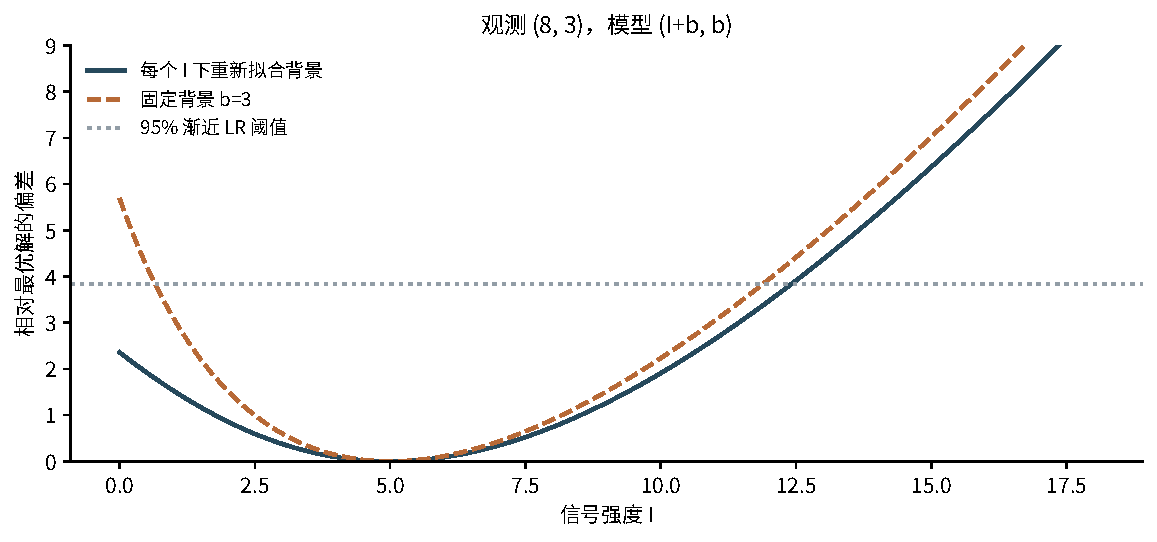
\includegraphics[width=0.95\textwidth]{figures/05_poisson_profile.pdf}
\caption{上述两像素例子的条件剖面偏差。虚线背景固定在 3；实线允许背景重新拟合。水平线采用单参数 95\% 渐近阈值，仅用于展示区间机制。}
\end{figure}

带读出噪声的 ADU 不等于整数光子计数。原有 Ariadne 保留泊松--高斯卷积似然；新分流器检查噪声来源、增益和读出方差声明，卷积后端另要求明确的已去偏置标记。它们不能因为信号弱就自动把 ADU 当成纯泊松计数。
